\documentclass[11pt]{article}
\usepackage{algorithm2e}
\usepackage[bottom]{footmisc} 
\usepackage[italian]{babel}
\usepackage[document]{ragged2e}
\usepackage{tabularx}
\justifying
\usepackage{amsfonts, amssymb, amsmath}
\usepackage{cancel}
\usepackage{float}
\usepackage{mathtools}
\usepackage[margin=2cm]{geometry}
% \setcounter{secnumdepth}{0}
\usepackage{hyperref}
\hypersetup{
    colorlinks,
    citecolor=black,
    filecolor=black,
    linkcolor=black,
    urlcolor=black
}
\usepackage{array}
\usepackage{makecell}
\usepackage{hyperref}
\usepackage[noabbrev,capitalize,italian]{cleveref}
\newcommand{\fref}[1]{\hyperref[#1]{\cref{#1}}}
\usepackage{makecell}
\usepackage{etoolbox}
\patchcmd{\thebibliography}{\section*{\refname}}{}{}{}
\usepackage{enumitem}

\tolerance=1
\emergencystretch=\maxdimen
\hyphenpenalty=10000
\hbadness=10000

\begin{document}
\begin{titlepage}
    \begin{center}
        \vspace*{1.5cm}
            
        \Huge
        \textbf{Campionato di\\gare automobilistiche}
            
        \vspace{0.3cm}
        \LARGE
        Report\\[0.2em]

        \vspace{1.5cm}
          
        \begin{minipage}[t]{0.47\textwidth}
            \begin{center}
                \parbox{65mm}{\centering\large {\bf Cheikh Ibrahim $\cdot$ Zaid} \\[0.3em] Matricola: \texttt{0000974909} \\[0.3em] \href{mailto:zaid.cheikhibrahim@studio.unibo.it}{\textit{zaid.cheikhibrahim@studio.unibo.it}}} \\[2em]
            \end{center}
		\end{minipage}
		\hfill
		\begin{minipage}[t]{0.47\textwidth}\raggedleft
            \begin{center}
                \parbox{65mm}{\centering\large {\bf Xia $\cdot$ Tian Cheng} \\[0.3em] Matricola: \texttt{0000975129} \\[0.3em] \href{mailto:tiancheng.xia@studio.unibo.it}{\textit{tiancheng.xia@studio.unibo.it}}} \\[2em]
            \end{center}
		\end{minipage}  
            
        \vspace{9cm}
            
        Anno accademico\\
        $2022 - 2023$
            
        \vspace{0.8cm}
            
            
        \Large
        Corso di Basi di dati\\
        Alma Mater Studiorum $\cdot$ Università di Bologna\\
            
    \end{center}
\end{titlepage}
\pagebreak


\tableofcontents
\newpage


\section{Analisi dei requisiti}
\subsection{Requisiti espressi in linguaggio naturale \textbf{RIFRASARE IN FUTURO, E' GIUSTIFICATO IL TESTO?}}
Si vuole realizzare un database per gestire un campionato di gare automobilistiche. \\
È necessario codificare le gare, le piste su cui si svolgono, i dati relativi ai giri, eventuali infrazioni e i dati sui pit stop. \\
Inoltre, si vogliono memorizzare i dati dei piloti che partecipano e i contratti (presenti e passati) che stipulano con le scuderie. Oltre ai dati relativi alle scuderie, è richiesto registrarne le auto e i meccanici. \\
Infine, si vuole tenere traccia dei controlli di regolarità effettuati dai supervisori (della società che organizza il campionato) e dei dati degli sponsor delle gare e delle singole scuderie. \\[1em]

Per le gare si vuole memorizzare il nome, la data di svolgimento, la pista su cui si corre, il numero di giri previsti, i piloti partecipanti e l'eventuale sponsor. \\
Per le piste si vogliono rappresentare il nome, la nazione e la città di collocazione, la lunghezza (in metri), numero di posti a sedere per gli spettatori. \\
Per i giri si vogliono salvare il tempo impiegato (in secondi), il numero del giro, la gara di appartenenza, il pilota che effettua il giro. \\
Per le infrazioni si vogliono gestire i dati riguardanti il nome e la descrizione e vengono assegnate ad un giro di un pilota sottoforma di penalità (in secondi). \\
Per i pit stop si vogliono rappresentare il tempo delle operazioni, il tempo complessivo (tempo di entrata e uscita + tempo delle operazioni), il giro in cui viene il pilota che viene chiamato ai box e i meccanici che effettuano le operazioni. \\
Per i piloti si vogliono memorizzare il nome, cognome, luogo e data di nascita. \\
Per i contratti si vogliono rappresentare il numero identificativo, il pilota ed il suo numero identificativo, la scuderia, la data d'inizio e di fine, l'auto assegnata e il valore di ingaggio. \\
Per le scuderie si vogliono gestire i dati riguardo la ragione sociale, la nazione della sede principale, l'anno di fondazione, il colore caratterizzante e i vari sponsor. \\ 
Per le auto si vogliono salvare la potenza (in cavalli), velocità massima raggiungibile, la scuderia di appartenenza. \\
Per i meccanici si vogliono memorizzare il nome, cognome, luogo, data di nascita, il ruolo e la scuderia di appartenenza. \\
Per i controlli di regolarità si vogliono tracciare i dati riguardo la data e l'ora, l'auto coinvolta, il supervisore e l'esito. \\
Per i supervisori si vogliono memorizzare il nome, cognome, luogo, data di nascita. \\
Per gli sponsor si vogliono salvare la ragione sociale, la tipologia di azienda, il capitale investito e la nazione della sede principale.

\subsection{Glossario dei termini \textbf{RIVEDERE COLLEGAMENTI}}
\begin{tabularx}{\linewidth}{
        |>{\hsize=0.9\hsize}X|% 10% of 4\hsize 
        >{\hsize=1.8\hsize}X|% 30% of 4\hsize
        >{\hsize=0.6\hsize}X|% 30% of 4\hsize 
        >{\hsize=0.7\hsize}X|% 30% of 4\hsize
           % sum=4.0\hsize for 4 columns
    }
    \hline
    \textbf{Termine} & \textbf{Descrizione} & \textbf{Sinonimi} & \textbf{Collegamenti} \\
    \hline
    Società organizzante & Azienda che organizza un campionato & - & \\
    \hline
    Campionato & Numero definito di gare con classifica & - & Gare \\
    \hline
    Gare & Competizione in cui partecipa un numero fissato di piloti che effettuano un numero definito di giri di pista sul proprio veicolo & Competizione & Piste, giri, piloti, sponsor \\
    \hline
    Giri & Percorrenza intera di una pista effettuata da un pilota & - & Pilota, gara \\
    \hline
    Piste & Località asfaltata idonea al passaggio di veicoli ad elevata velocità & - & \\
    \hline
    Infrazioni & Eventi irregolari accaduti durante una gara & - & Penalità, giro, pilota \\
    \hline
    Penalità & Tempo ulteriore assegnato come malus al tempo totale & - & \\
    \hline
    Veicolo & Autoveicolo ad elevata velocità & Auto & Scuderia \\
    \hline
    Piloti & Persona che guida un veicolo ad elevata velocità & - & \\
    \hline
    Scuderie & Azienda proprietaria di veicoli & - & Sponsor \\
    \hline
    Meccanici & Impiegati delle scuderie adibiti alla manutenzione dell'auto & - & Scuderia \\
    \hline
    Supervisori & Impiegati della società organizzante adibiti ai controlli di regolarità & - & \\
    \hline
    Controlli di regolarità & Controlli effettuati dalla società organizzatrice per garantire la regolarità dei veicoli & Controlli & Supervisore \\
    \hline
    Sponsor & Azienda che investe per apparire in gare e/o in scuderie & - & \\
    \hline
    Pit stop & Fase di un giro in cui l'auto sosta in un'apposita area di pista dove i meccanici effettuano operazioni all'auto & - & Giro, pilota, meccanici \\
    \hline
    Contratto & Accordo stipulato tra un pilota e una scuderia per gareggiare in un campionato & - & Pilota, scuderia \\
    \hline
\end{tabularx}

\subsection{Eliminazione delle ambiguità presenti}
\subsection{Strutturazione dei requisiti}
\subsection{Specifica operazioni}
\begin{enumerate}
    \item Inserire una nuova scuderia (in media 1 volta ogni cinque anni)
    \item Inserire una nuova gara (in media 1 volta all'anno)
    \item Inserire il tempo pit stop ($\sim$20 volte per gara)
    \item Inserire il tempo di un giro del pilota sulla pista ($\sim$1000 volte per gara)
    \item Inserire un nuovo contratto tra pilota e scuderia (poche volte ogni anno)
    \item Visualizzare lo sponsor di una gara (1 volta per gara)
    \item Visualizzare il pilota con il tempo migliore su una data pista (1 volta per gara)
    \item Visualizzare i piloti e la scuderia con cui gareggiano per una data gara ordinandoli per scuderia (1 volta per gara)
    \item Visualizzare la classifica (finale o temporanea) di una data gara ($\sim$50 volte per gara)
    \item Visualizzare il pilota con il maggior numero di vittorie (1 volta per gara)
    \item Visualizzare la scuderia con il maggior numero di vittorie (1 volta per gara)
    \item Visualizzare lo sponsor più presente (1 volta all'anno)
    \item Visualizzare la scuderia con cui un pilota ha un contratto in una determinata data (poche volte all'anno)
    \item Visualizzare nome, cognome e numero dei piloti di una data scuderia con contratto attivo al momento attuale (poche volte all'anno)
\end{enumerate}

\section{Progettazione concettuale}
È stato seguito un approccio bottom-up per definire i macro-argomenti.\\
Sono quindi state individuate le seguenti categorie:
\begin{itemize}
    \item Persone
    \item Aziende
    \item Partecipanti: cattura i concetti relativi alle scuderie e ai piloti.
    \item Competizione: cattura i concetti relativi allo svolgimento della gara.
\end{itemize}
\subsection{Identificazione delle entità e relazioni}

\subsection{Definizioni delle entità generalizzabili}
Le entità generalizzabili sono le persone e le aziende.
\subsubsection{Definizioni delle persone}
Come persone, sono state identificate le entità supervisori, piloti e meccanici. 
\begin{figure}[H]
    \centering
    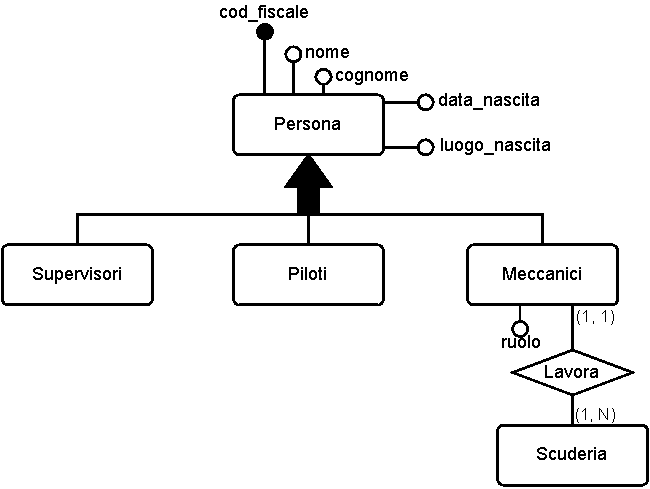
\includegraphics[width=10cm]{../er/gare_persone.pdf}
\end{figure}

\subsubsection{Definizioni delle aziende}
Come aziende, sono state identificate le entità scuderia e sponsor. 
\begin{figure}[H]
    \centering
    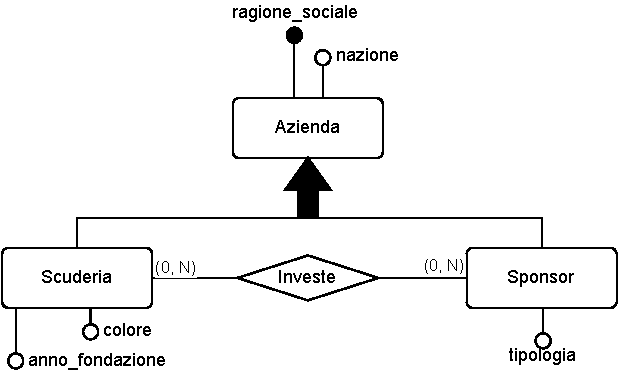
\includegraphics[width=10cm]{../er/gare_aziende.pdf}
\end{figure}

\subsection{Definizioni dei macro-argomenti}
\subsubsection{Definizioni dei partecipanti}
Riguardo i partecipanti, con approccio inside-out, sono state identificate le entità: scuderia, contratto, auto, controllo. Oltre a pilota, meccanico, supervisore, sponsor.
\begin{figure}[H]
    \centering
    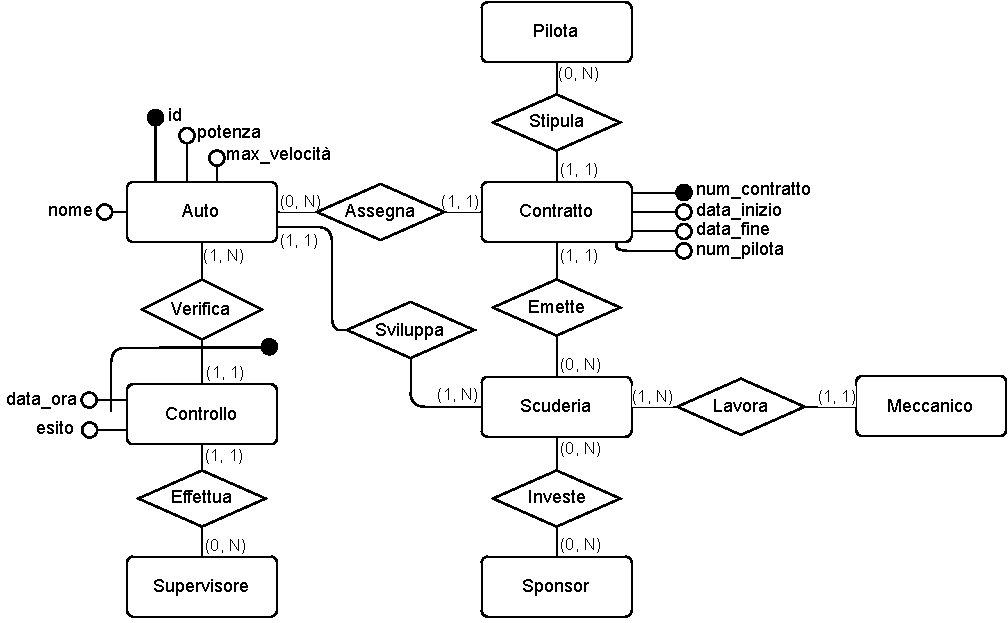
\includegraphics[width=15.5cm]{../er/gare_scuderie.pdf}
\end{figure}

\subsubsection{Definizioni delle competizioni}
Per il concetto di competizione sono state identificate con approccio inside-out le entità: gara, pista, giro, infrazione, pit stop. Oltre a pilota, meccanico, sponsor.
\begin{figure}[H]
    \centering
    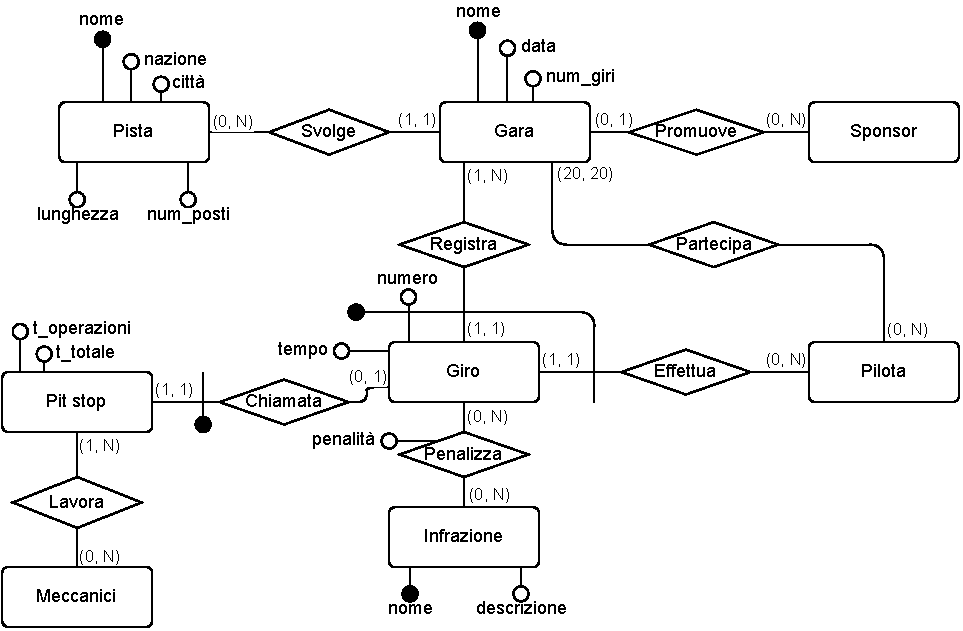
\includegraphics[width=15.5cm]{../er/gare_gara.pdf} % TODO CORREGGERE ENTITA' MECCANICI->MECCANICO !!!!!!!!!!!!!!!!!!!!!!!!!!!!!!!
\end{figure}                                            % I MECCANICI HANNO UN RUOLOOOOOOOOOOOO

\subsection{Schema finale}
\begin{figure}[H]
    \centering
    \makebox[0cm]{
        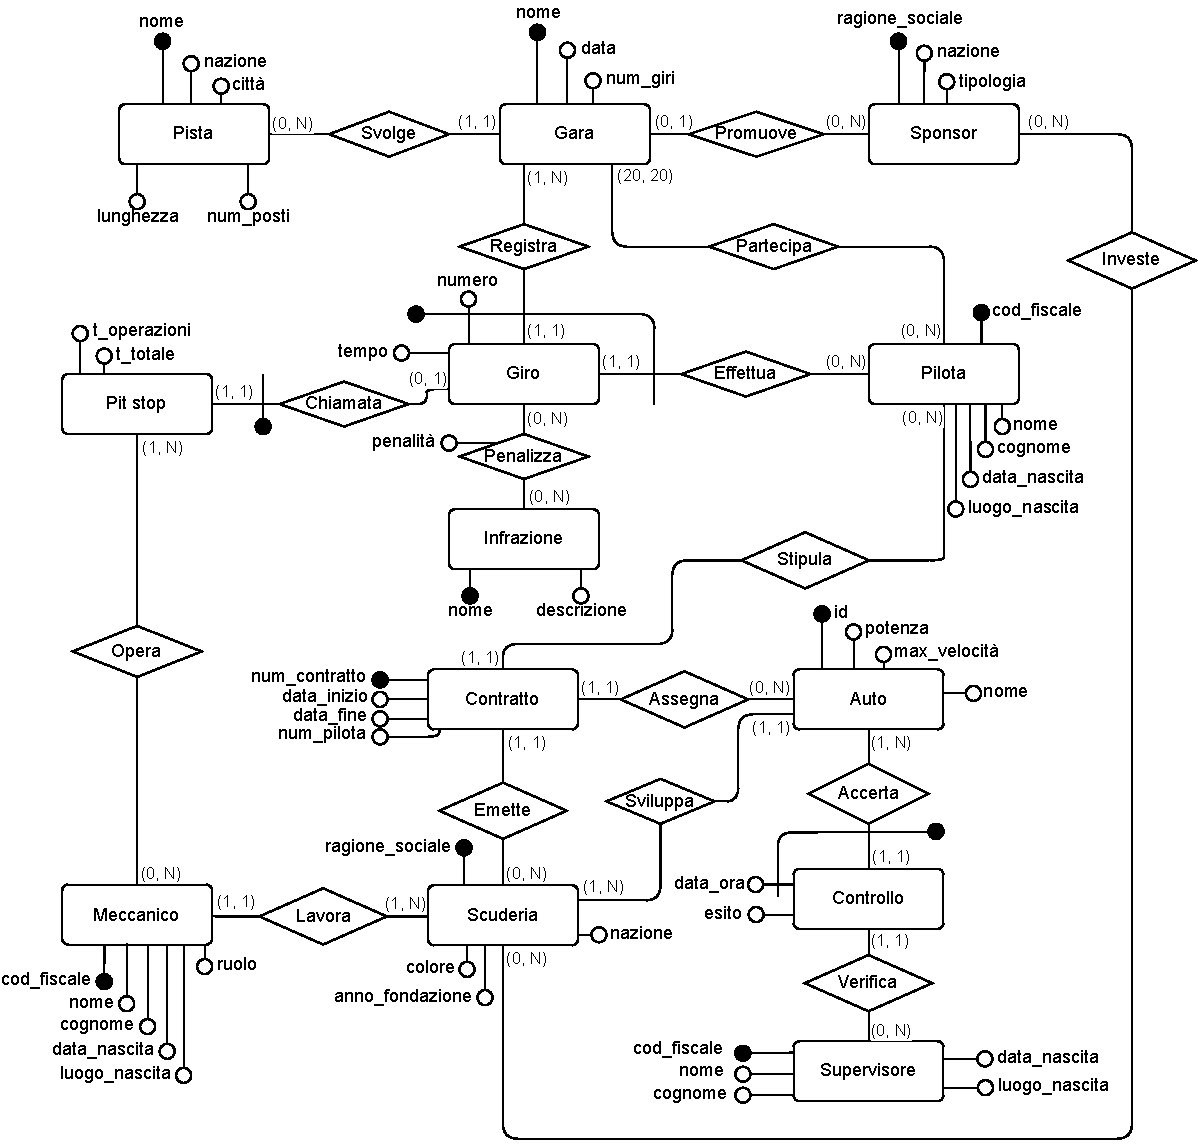
\includegraphics[width=18cm]{../er/gare.pdf}
    }
\end{figure}


\subsection{Dizionario dei dati}

\begin{center}
\makebox[0cm]{
    \begin{tabular}{ |l|p{5.5cm}|p{5cm}|p{4cm}| }
        \hline
        \textbf{Nome entità} & \textbf{Descrizione} & \textbf{Attributi} & \textbf{Identificatore} \\
        
        \hline
        Pilota & 
        Persona che guida un veicolo & 
        \parbox[t]{\linewidth}{Nome (stringa)\\Cognome (stringa)\\Data di nascita (data)\\Luogo di nascita (stringa)} & 
        Codice fiscale (stringa) \\
        
        \hline
        Meccanico &
        Persona che opera su un veicolo & 
        \parbox[t]{\linewidth}{Nome (stringa)\\Cognome (stringa)\\Data di nascita (data)\\Luogo di nascita (stringa)\\Ruolo (stringa)} & 
        Codice fiscale (stringa) \\

        \hline
        Supervisore &
        Persona che effettua dei controlli di regolarità per conto della società organizzante & 
        \parbox[t]{\linewidth}{Nome (stringa)\\Cognome (stringa)\\Data di nascita (data)\\Luogo di nascita (stringa)} & 
        Codice fiscale (stringa) \\

        \hline
        Scuderia &
        Azienda che stipula contratti con piloti e crea auto da corsa & 
        \parbox[t]{\linewidth}{Colore (stringa)\\Nazione (stringa)\\Anno di fondazione (numero)} & 
        Ragione sociale (stringa) \\

        \hline
        Sponsor &
        Azienda che investe in gare e scuderie & 
        \parbox[t]{\linewidth}{Tipologia (stringa)\\Nazione (stringa)} & 
        Ragione sociale (stringa) \\
        
        \hline
        Contratto &
        Documento stipulato tra un pilota e una scuderia & 
        \parbox[t]{\linewidth}{Data inizio (data)\\Data fine (data)\\Numero pilota (numero)} & 
        Numero contratto (stringa) \\

        \hline
        Auto &
        Autovettura ad elevata velocità di fabbricazione di una scuderia guidata da un pilota &
        \parbox[t]{\linewidth}{Potenza (numero)\\Velocità massima (numero)} & 
        Id (stringa) \\

        \hline
        Controllo &
        Verifica della regolarità di un auto effettuata da un supervisore & 
        \parbox[t]{\linewidth}{Esito (Booleano)} & 
        \parbox[t]{\linewidth}{Data e ora (data)\\Id [Auto] } \\

        \hline
        Gara &
        Competizione dove 20 piloti gareggiano su una pista un numero di giri prestabilito & 
        \parbox[t]{\linewidth}{Data (data)\\Numero giri (numero)} & 
        Nome (stringa) \\

        \hline
        Pista &
        Località asfaltata adatta a ospitare gare ad alta velocità & 
        \parbox[t]{\linewidth}{Nazione (stringa)\\Città (stringa)\\Lunghezza (numero)\\Numero posti (numero)} & 
        Nome (stringa) \\

        \hline
        Giro &
        Singola percorrenza completa di pista & 
        \parbox[t]{\linewidth}{Tempo (numero)} & 
        \parbox[t]{\linewidth}{Numero (numero)\\Nome [Gara]\\Codice fiscale [Pilota]} \\ 

        \hline
        Infrazione &
        Evento irregolare durante una gara & 
        \parbox[t]{\linewidth}{Descrizione (stringa)} & 
        Nome (stringa) \\

        \hline
        Pit stop &
        Fase di gara dove l'auto sosta in una specifica area di pista per permettere ai meccanici di effettuare piccole modifiche & 
        \parbox[t]{\linewidth}{Tempo operazioni (numero)\\Tempo totale (numero)} & 
        Chiavi di [Giro] \\

        \hline
    \end{tabular}
}
\end{center}

\begin{center}
    \makebox[0cm]{
        \begin{tabular}{ |l|p{5.5cm}|p{5cm}|p{4cm}| }
            \hline
            \textbf{Nome relazione} & \textbf{Descrizione} & \textbf{Entità coinvolte} & \textbf{Attributi} \\
            
            \hline
            Svolge & 
            Associa la pista su cui si svolge una gara & 
            \parbox[t]{\linewidth}{Pista (0, N)\\Gara (1, 1)} & 
            \parbox[t]{\linewidth}{-} \\

            \hline
            Promuove & 
            Associa l'eventuale sponsor che promuove una gara & 
            \parbox[t]{\linewidth}{Gara (0, 1)\\Sponsor (0, N)} & 
            \parbox[t]{\linewidth}{-} \\

            \hline
            Registra & 
            Associa un giro effettuato in una gara & 
            \parbox[t]{\linewidth}{Gara (1, N)\\Giro (1, 1)} & 
            \parbox[t]{\linewidth}{-} \\

            \hline
            Partecipa & 
            Associa un pilota che partecipa ad una gara & 
            \parbox[t]{\linewidth}{Gara (20, 20)\\Pilota (0, N)} & 
            \parbox[t]{\linewidth}{-} \\

            \hline
            Investe & 
            Associa l'eventuale sponsor che investe in una o più scuderie & 
            \parbox[t]{\linewidth}{Sponsor (0, N)\\Scuderia (0, N)} & 
            \parbox[t]{\linewidth}{-} \\

            \hline
            Chiamata & 
            Associa il giro in cui il pilota viene chiamato per il pit stop & 
            \parbox[t]{\linewidth}{Pit stop (1, 1)\\Giro (0, 1)} & 
            \parbox[t]{\linewidth}{-} \\

            \hline
            Effettua & 
            Associa il giro che viene effettuato dal pilota & 
            \parbox[t]{\linewidth}{Giro (1, 1)\\Pilota (0, N)} & 
            \parbox[t]{\linewidth}{-} \\

            \hline
            Penalizza & 
            Associa la penalità al giro in cui viene commessa l'infrazione & 
            \parbox[t]{\linewidth}{Giro (0, N)\\Penalità (0, N)} & 
            \parbox[t]{\linewidth}{Penalità (numero)} \\

            \hline
            Opera & 
            Associa i meccanici che lavorano durante la sosta al pit stop & 
            \parbox[t]{\linewidth}{Pit stop (1, N)\\Meccanico (0, N)} & 
            \parbox[t]{\linewidth}{-} \\

            \hline
            Stipula & 
            Associa il contratto firmato da un pilota & 
            \parbox[t]{\linewidth}{Pilota (0, N)\\Contratto (1, 1)} & 
            \parbox[t]{\linewidth}{-} \\

            \hline
            Assegna & 
            Associa l'auto assegnata nel contratto & 
            \parbox[t]{\linewidth}{Contratto (1, 1)\\Auto (0, N)} & 
            \parbox[t]{\linewidth}{-} \\

            \hline
            Emette & 
            Associa la scuderia ai contratti che emette & 
            \parbox[t]{\linewidth}{Contratto (1, 1)\\Scuderia (0, N)} & 
            \parbox[t]{\linewidth}{-} \\

            \hline
            Lavora & 
            Associa un meccanico a una scuderia per la quale lavora & 
            \parbox[t]{\linewidth}{Meccanico (1, 1)\\Scuderia (1, N)} & 
            \parbox[t]{\linewidth}{-} \\

            \hline
            Accerta & 
            Associa un controllo che viene effettuato su un'auto & 
            \parbox[t]{\linewidth}{Auto (1, N)\\Controllo (1, 1)} & 
            \parbox[t]{\linewidth}{-} \\
            
            \hline
            Verifica & 
            Associa un controllo che viene effettuato da un supervisore & 
            \parbox[t]{\linewidth}{Controllo (1, 1)\\Supervisore (0, N)} & 
            \parbox[t]{\linewidth}{-} \\
            
            \hline
        \end{tabular}
    }
\end{center}

\subsection{Regole aziendali [RIVEDERE]}
\subsubsection{Regole di vincolo}
\begin{enumerate}[label={RV \arabic*}, leftmargin=4em]
    \item Il numero di giri di una gara deve essere $>0$.
    \item Data una gara, il numero di giri effettuato da un pilota, deve essere al più il numero di giri della gara.\\
          Il numero di un giro deve essere quindi compreso tra $[1, \text{numero di giri della gara}]$.
    \item Il numero di posti e la lunghezza di una pista devono essere $>0$. 
    \item Il tempo di un giro deve essere essere $>0$. 
    \item Il tempo delle operazioni e tempo totale dei pit stop devono essere $>0$.
    \item Il tempo della penalità deve essere $>0$.
    \item La potenza e la velocità massima di un'auto deve essere $>0$.
    \item In un dato istante, un pilota può avere attivo un solo contratto con una scuderia.
    \item La data di inizio di un contratto deve essere antecedente alla data di fine.
    \item I meccanici che operano ad un pit stop devono appartenere alla stessa scuderia del pilota che effettua il giro.
    \item Un contratto deve avere come inizio una data antecedente a quella della fondazione della scuderia.
\end{enumerate}

% \subsubsection{Regole di derivazione}
% \begin{enumerate}[label={RD \arabic*}, leftmargin=4em]
%     \item 
% \end{enumerate}

\section{Progettazione logica}
% TODO CREARE ID IN GIRO AL POSTO DELLA CHIAVE GIGANTE
\subsection{Tavole dei volumi}
\begin{center}
    \begin{tabular}{ |l|l|l| }
        \hline
        \textbf{Concetto} & \textbf{Tipo} & \textbf{Volume} \\
        
        \hline
        Pilota & Entità & 30 \\
        \hline
        Meccanico & Entità & 150 \\
        \hline
        Supervisore & Entità & 15 \\
        \hline
        Scuderia & Entità & 10 \\
        \hline
        Sponsor & Entità & 50 \\
        \hline
        Contratto & Entità & 1400 \\
        \hline
        Auto & Entità & 20 \\
        \hline
        Controllo & Entità & 55000 \\ % (73 anni di F1 * 20 piloti per gara * 2 (un controllo a inizio gara e uno alla fine) * 20 gare in media per stagione)
        \hline
        Gara & Entità & 1100 \\
        \hline
        Pista & Entità & 50 \\
        \hline
        Giro & Entità & 70000 \\ % (73 anni di F1 * 20 gare in media per stagione * 50 giri in media per gara)
        \hline
        Infrazione & Entità & 20 \\
        \hline
        Pit stop & Entità & 20000 \\
        \hline
    \end{tabular}
        \quad
    \begin{tabular}{ |l|l|l| }
        \hline
        \textbf{Concetto} & \textbf{Tipo} & \textbf{Volume} \\

        \hline
        Svolge & Relazione & 1100 \\
        \hline
        Promuove & Relazione & 700 \\
        \hline
        Registra & Relazione & 70000 \\
        \hline
        Partecipa & Relazione & 22000 \\
        \hline
        Investe & Relazione & 300 \\
        \hline
        Chiamata & Relazione & 20000 \\
        \hline
        Effettua & Relazione & 70000 \\
        \hline
        Penalizza & Relazione & 8000 \\
        \hline
        Opera & Relazione & 300000 \\ % (volume meccanici 15 * volume pit stop 20000)
        \hline
        Stipula & Relazione & 1400 \\
        \hline
        Assegna & Relazione & 1400 \\
        \hline
        Emette & Relazione & 1400 \\
        \hline
        Lavora & Relazione & 150 \\
        \hline
        Accerta & Relazione & 55000 \\
        \hline
        Verifica & Relazione & 55000 \\
        \hline
    \end{tabular}
\end{center}

\subsection{Tavola delle operazioni}
\begin{center}
    \begin{tabular}{ |l|l| }
        \hline
        \textbf{Operazione} & \textbf{Frequenza} \\

        \hline
        1 & 1 volta ogni cinque anni \\
        \hline
        2 & 1 volta all'anno \\
        \hline
        3 & $\sim$20 volte per gara \\
        \hline
        4 & $\sim$1000 volte per gara \\
        \hline
        5 & Poche volte ogni anno \\
        \hline
        6 & 1 volta per gara \\
        \hline
        7 & 1 volta per gara \\
        \hline
        8 & 1 volta per gara \\
        \hline
        9 & $\sim$50 volte per gara \\
        \hline
        10 & 1 volta per gara \\
        \hline
        11 & 1 volta per gara \\
        \hline
        12 & 1 volta all'anno \\
        \hline
        13 & Poche volte all'anno \\
        \hline
    \end{tabular}
\end{center}

\subsection{Ristrutturazione dello schema concettuale}
\subsubsection{Cambio chiave per l'entità Giro}
La chiave dell'entità Giro comprende l'insieme degli attributi numero del giro, nome della gara e id del pilota. Inoltre, l'entità Pit stop utilizza come chiave l'associazione a Giro.\\
Tale approccio rende scomodo lavorare con le due entità, per tale ragione è stato deciso di introdurre un identificatore per l'entità Giro che svolge la funzione di chiave.

%
% Penalità ha ora come PRIMARY KEY un id
%

\subsection{Normalizzazione}
\subsection{Traduzione verso il modello relazionale}
% CAMBIARE AUTO IN VEICOLO PERCHE' PAROLA RISERVATA
\begin{center}
    \makebox[0cm]{
        \def\arraystretch{1.2}%
        \begin{tabular}{ |l|l| }
            \hline
            \textbf{Entità - Relazione} & \textbf{Traduzione} \\

            \hline
            Pilota & Pilota(\underline{codice\_fiscale}, nome, cognome, data\_nascita, luogo\_nascita) \\
            \hline
            Meccanico & \makecell[l]{Meccanico(\underline{codice\_fiscale}, nome, cognome,\\data\_nascita, luogo\_nascita, ruolo, scuderia)} \\
            \hline
            Supervisore & Supervisore(\underline{codice\_fiscale}, nome, cognome, data\_nascita, luogo\_nascita) \\
            \hline
            Scuderia & Scuderia(\underline{ragione\_sociale}, colore, nazione, anno\_fondazione) \\
            \hline
            Sponsor & Sponsor(\underline{ragione\_sociale}, tipologia, nazione) \\
            \hline
            Contratto & Contratto(\underline{numero}, data\_inizio, data\_fine, numero\_pilota, pilota, scuderia, auto) \\
            \hline
            Auto & Auto(\underline{id}, potenza, max\_velocita) \\
            \hline
            Controllo & Controllo(\underline{auto}, \underline{data\_ora}, esito, supervisore) \\
            \hline
            Gara & Gara(\underline{nome}, data, num\_giri, sponsor, pista) \\
            \hline
            Pista & Pista(\underline{nome}, nazione, citta, lunghezza, num\_posti) \\
            \hline
            Giro & Giro(\underline{id}, numero, tempo, gara, pilota) \\
            \hline
            Infrazione & Infrazione(\underline{nome}, descrizione) \\
            \hline
            Pit stop & Pitstop(\underline{giro}, tempo\_operazione, tempo\_totale) \\
            \hline
            Svolge & Accorpato in Gara \\
            \hline
            Promuove & Accorpato in Gara \\
            \hline
            Registra & Accorpato in Giro \\
            \hline
            Partecipa & Partecipa(\underline{gara}, \underline{pilota}) \\
            \hline
            Investe & Investe(\underline{sponsor}, \underline{scuderia}) \\
            \hline
            Chiamata & Accorpata in Pit Stop \\
            \hline
            Effettua & Accorpata in Giro \\
            \hline
            Penalizza & Penalizza(\underline{giro}, \underline{infrazione}, penalita) \\
            \hline
            Opera & Opera(\underline{pitstop}, \underline{meccanico}) \\
            \hline
            Stipula & Accorpato in Contratto \\
            \hline
            Assegna & Accorpato in Contratto \\
            \hline
            Emette & Accorpato in Contratto \\
            \hline
            Lavora & Accorpato in Meccanico \\
            \hline
            Accerta & Accorpato in Controllo \\
            \hline
            Verifica & Accorpato in Controllo \\
            \hline
        \end{tabular}
    }
\end{center}

\begin{center}
    \makebox[0cm]{
        \def\arraystretch{1.2}%
        \begin{tabular}{ |l|l| }
            \hline
            \textbf{Entità - Relazione} & \textbf{Traduzione} \\

            \hline
            Pilota(\underline{codice\_fiscale}, nome, cognome, data\_nascita, luogo\_nascita) & \makecell[l]{-} \\
            \hline
            \makecell[l]{Meccanico(\underline{codice\_fiscale}, nome, cognome,\\data\_nascita, luogo\_nascita, ruolo, scuderia)} & \makecell[l]{scuderia $\rightarrow$ Scuderia.ragione\_sociale} \\
            \hline
            \makecell[l]{Supervisore(\underline{codice\_fiscale}, nome, cognome,\\data\_nascita, luogo\_nascita)} & \makecell[l]{-} \\
            \hline
            Scuderia(\underline{ragione\_sociale}, colore, nazione, anno\_fondazione) & \makecell[l]{-} \\
            \hline
            Sponsor(\underline{ragione\_sociale}, tipologia, nazione) & \makecell[l]{-} \\
            \hline
            \makecell[l]{Contratto(\underline{numero}, data\_inizio, data\_fine,\\numero\_pilota, pilota, scuderia, veicolo)} & \makecell[l]{pilota $\rightarrow$ Pilota.codice\_fiscale \\ scuderia $\rightarrow$ Scuderia.ragione\_sociale \\ auto $\rightarrow$ Auto.id} \\
            \hline
            Veicolo(\underline{id}, nome, potenza, max\_velocita) & \makecell[l]{-} \\ % AGGIORNARE ER -> E' STATO AGGIUNTO IL CAMPO NOME
            \hline
            Controllo(\underline{veicolo}, \underline{data\_ora}, esito, supervisore) & \makecell[l]{veicolo $\rightarrow$ Veicolo.id\\supervisore $\rightarrow$ Supervisore.codice\_fiscale} \\
            \hline
            Gara(\underline{nome}, data\_ora, num\_giri, sponsor, pista) & \makecell[l]{sponsor $\rightarrow$ Sponsor.ragione\_sociale \\ pista $\rightarrow$ Pista.nome} \\
            \hline
            Pista(\underline{nome}, nazione, citta, lunghezza, num\_posti) & \makecell[l]{-} \\
            \hline
            Giro(\underline{id}, numero, tempo, gara, pilota) & \makecell[l]{gara $\rightarrow$ Gara.nome \\ pilota $\rightarrow$ Pilota.codice\_fiscale} \\
            \hline
            Infrazione(\underline{nome}, descrizione) & \makecell[l]{-} \\
            \hline
            Pitstop(\underline{giro}, tempo\_operazione, tempo\_totale) & \makecell[l]{giro $\rightarrow$ Giro.id} \\
            \hline
            Partecipa(\underline{gara}, \underline{pilota}) & \makecell[l]{gara $\rightarrow$ Gara.nome \\ pilota $\rightarrow$ Pilota.codice\_fiscale} \\
            \hline
            Investe(\underline{sponsor}, \underline{scuderia}) & \makecell[l]{sponsor $\rightarrow$ Sponsor.ragione\_sociale \\ scuderia $\rightarrow$ Scuderia.ragione\_sociale } \\
            \hline
            Penalizza(\underline{giro}, \underline{infrazione}, penalita) & \makecell[l]{giro $\rightarrow$ Giro.id \\ infrazione $\rightarrow$ Infrazione.nome} \\
            \hline
            Opera(\underline{pitstop}, \underline{meccanico}) & \makecell[l]{pitstop $\rightarrow$ Pitstop.giro \\ meccanico $\rightarrow$ Meccanico.codice\_fiscale} \\
            \hline
        \end{tabular}
    }
\end{center}



\section{Codifica SQL}
\subsection{Definizione dello schema}
\subsection{Codifica delle operazioni}


\section{Testing}

\end{document}
